% =====================================================================
%  Combined architecture comparison -- TikZ matrix (vertical stack).
%  Each pipeline is a wide horizontal flow, so stacking at full width keeps
%  the labels legible; the bold (a)/(b)/(c) tags provide the sub-labels.
%  Requires the three sibling PDFs to be compiled first:
%     pdflatex arch_no_video.tex
%     pdflatex arch_global_video.tex
%     pdflatex arch_agent_centric.tex
%     pdflatex arch_combined_all.tex
% =====================================================================
\documentclass[tikz, border=10pt]{standalone}
\usepackage{graphicx}
\usetikzlibrary{matrix, positioning}

\begin{document}
\begin{tikzpicture}
  \matrix (M) [
      matrix of nodes,
      row sep=6mm,
      column sep=5mm,
      nodes={anchor=center, font=\small},
    ] {
      \textbf{(a)} & 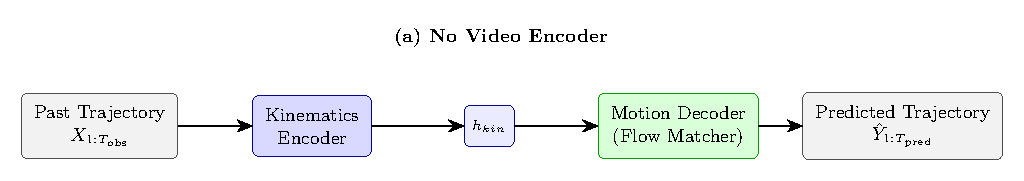
\includegraphics[width=15.5cm]{arch_no_video.pdf} \\
      \textbf{(b)} & 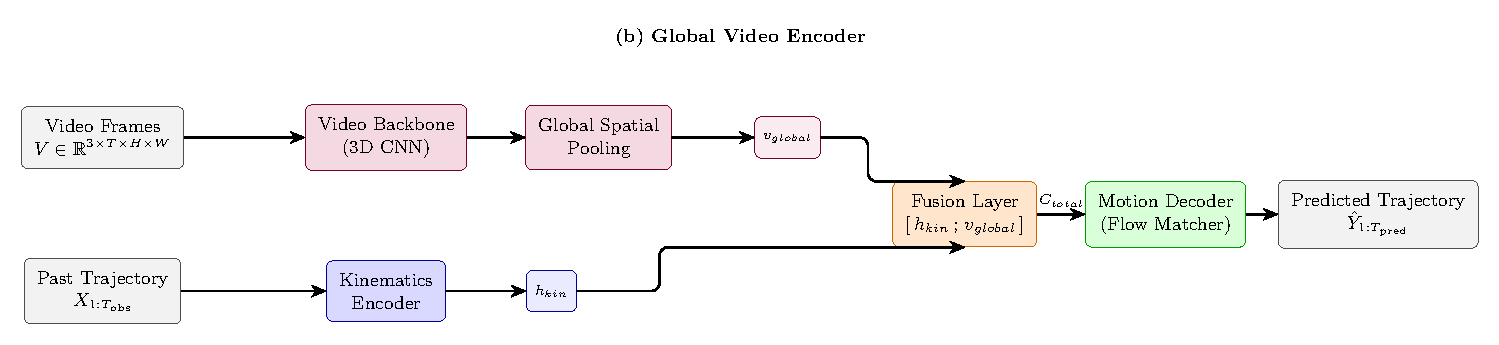
\includegraphics[width=15.5cm]{arch_global_video.pdf} \\
      \textbf{(c)} & 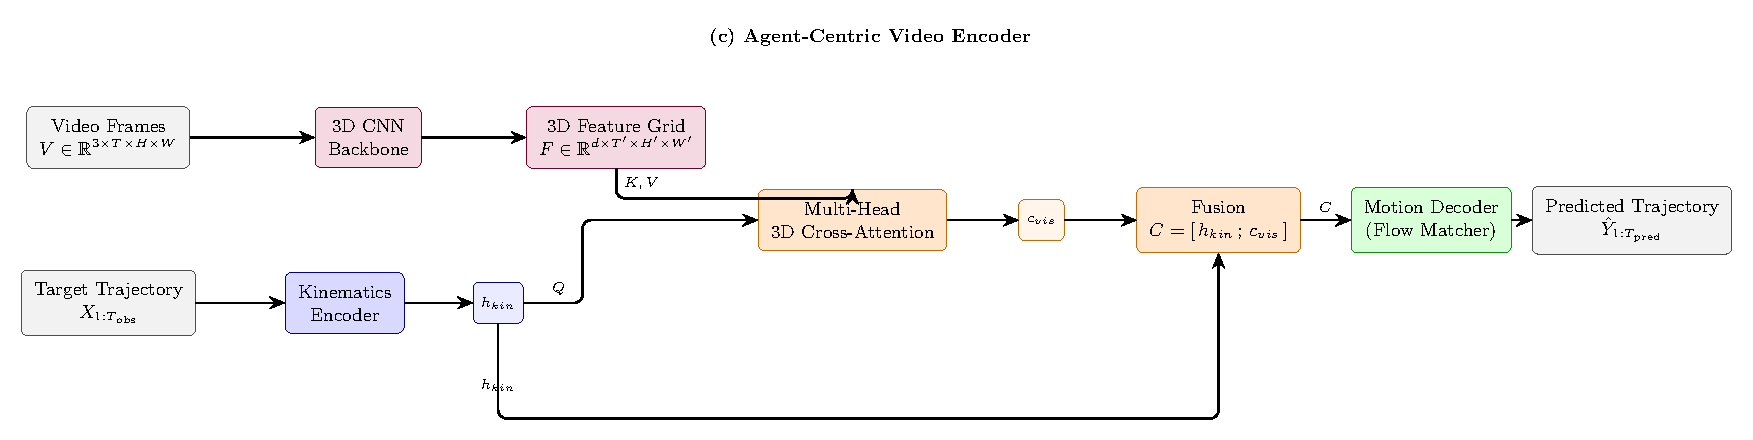
\includegraphics[width=15.5cm]{arch_agent_centric.pdf} \\
    };
\end{tikzpicture}
\end{document}
